\subsection{Fichier des meilleurs scores dans le jeu \q{Block out} et sérialisation basique}

De nombreux jeux vidéo ont un fichier des meilleurs scores, parfois appelé \q{Hall of fame}.
L'ancien jeu \q{Block out}\footnote{\url{http://www.bestoldgames.net/eng/old-games/blockout.php}}
(tetris 3D de 1989) ne fait pas exception, voici ce que nous voyons à la fin:

\begin{figure}[H]
\centering
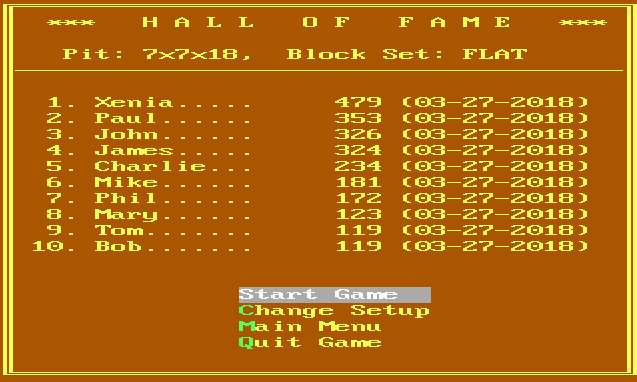
\includegraphics[width=0.7\textwidth]{advanced/550_more_structs/blockout/hs.png}
\caption{Table des meilleurs scores}
\end{figure}

Maintenant, nous pouvons voir que le fichier qui a changé après que nous ayons ajouté
notre nom est \IT{BLSCORE.DAT}.

\begin{lstlisting}
% xxd -g 1 BLSCORE.DAT

00000000: 0a 00 58 65 6e 69 61 2e 2e 2e 2e 2e 00 df 01 00  ..Xenia.........
00000010: 00 30 33 2d 32 37 2d 32 30 31 38 00 50 61 75 6c  .03-27-2018.Paul
00000020: 2e 2e 2e 2e 2e 2e 00 61 01 00 00 30 33 2d 32 37  .......a...03-27
00000030: 2d 32 30 31 38 00 4a 6f 68 6e 2e 2e 2e 2e 2e 2e  -2018.John......
00000040: 00 46 01 00 00 30 33 2d 32 37 2d 32 30 31 38 00  .F...03-27-2018.
00000050: 4a 61 6d 65 73 2e 2e 2e 2e 2e 00 44 01 00 00 30  James......D...0
00000060: 33 2d 32 37 2d 32 30 31 38 00 43 68 61 72 6c 69  3-27-2018.Charli
00000070: 65 2e 2e 2e 00 ea 00 00 00 30 33 2d 32 37 2d 32  e........03-27-2
00000080: 30 31 38 00 4d 69 6b 65 2e 2e 2e 2e 2e 2e 00 b5  018.Mike........
00000090: 00 00 00 30 33 2d 32 37 2d 32 30 31 38 00 50 68  ...03-27-2018.Ph
000000a0: 69 6c 2e 2e 2e 2e 2e 2e 00 ac 00 00 00 30 33 2d  il...........03-
000000b0: 32 37 2d 32 30 31 38 00 4d 61 72 79 2e 2e 2e 2e  27-2018.Mary....
000000c0: 2e 2e 00 7b 00 00 00 30 33 2d 32 37 2d 32 30 31  ...{...03-27-201
000000d0: 38 00 54 6f 6d 2e 2e 2e 2e 2e 2e 2e 00 77 00 00  8.Tom........w..
000000e0: 00 30 33 2d 32 37 2d 32 30 31 38 00 42 6f 62 2e  .03-27-2018.Bob.
000000f0: 2e 2e 2e 2e 2e 2e 00 77 00 00 00 30 33 2d 32 37  .......w...03-27
00000100: 2d 32 30 31 38 00                                -2018.
\end{lstlisting}

Toutes les entrées sont clairement visibles.
Le premier octet est probablement le nombre d'entrées.
Le second est zéro, en fait, le nombre d'entrées peut-être une valeurs 16-bit couvrant
les deux premiers octets.

Ensuite, après le nom \q{Xenia}, nous voyons les octets 0xDF et 0x01.
Xenia a un score de 479, et ceci est exactement 0x1DF en hexadécimal.
Donc une valeur de score est probablement un entier 16-bit, ou un entier 32-bit:
il y a deux octets à zéro de plus après.

Maintenant, pensons au fait qu'à la fois les éléments des tableaux et des structures
sont toujours placés en mémoire de manière adjacente les uns aux autres.
\myindex{\CStandardLibrary!write()}
\myindex{\CStandardLibrary!fwrite()}
\myindex{\CStandardLibrary!read()}
\myindex{\CStandardLibrary!fread()}
Cela nous permet d'écrire le tableau/la structure entièrement dans le fichier en
utilisant une fonction unique \IT{write()} ou \IT{fwrite()}, et de le restaurer en
utilisant \IT{read()} ou \IT{fread()}, aussi simplement que ça.
Ceci est ce qui est appelé \IT{sérialisation} de nos jours.

\subsubsection{Lire}

Maintenant, écrivons un petit programme en C pour lire le fichier des meilleurs scores:

\begin{lstlisting}[style=customc]
#include <assert.h>
#include <stdio.h>
#include <stdint.h>
#include <string.h>

struct entry
{
	char name[11]; // incl. terminating zero
	uint32_t score;
	char date[11]; // incl. terminating zero
} __attribute__ ((aligned (1),packed));

struct highscore_file
{
	uint8_t count;
	uint8_t unknown;
	struct entry entries[10];
} __attribute__ ((aligned (1), packed));

struct highscore_file file;

int main(int argc, char* argv[])
{
	FILE* f=fopen(argv[1], "rb");
	assert (f!=NULL);
	size_t got=fread(&file, 1, sizeof(struct highscore_file), f);
	assert (got==sizeof(struct highscore_file));
	fclose(f);
	for (int i=0; i<file.count; i++)
	{
		printf ("name=%s score=%d date=%s\n",
				file.entries[i].name,
				file.entries[i].score,
				file.entries[i].date);
	};
};
\end{lstlisting}

Nous avons besoin de l'attribut \IT{((aligned (1),packed))} de GCC afin que tous
les champs de la structure soient alignés sur une limite de 1-octet.

Bien sûr, il fonctionne:

\begin{lstlisting}
name=Xenia..... score=479 date=03-27-2018
name=Paul...... score=353 date=03-27-2018
name=John...... score=326 date=03-27-2018
name=James..... score=324 date=03-27-2018
name=Charlie... score=234 date=03-27-2018
name=Mike...... score=181 date=03-27-2018
name=Phil...... score=172 date=03-27-2018
name=Mary...... score=123 date=03-27-2018
name=Tom....... score=119 date=03-27-2018
name=Bob....... score=119 date=03-27-2018
\end{lstlisting}

(Inutile de dire que chaque nom est complété avec des points, à la fois à l'écran
et dans le fichier, peut-être pour des raisons esthétique.)

\subsubsection{Écrire}

Vérifions si nous avons raison à propos de la largeur d'une valeur de score. Est-ce
réellement sur 32 bits?

\begin{lstlisting}[style=customc]
int main(int argc, char* argv[])
{
	FILE* f=fopen(argv[1], "rb");
	assert (f!=NULL);
	size_t got=fread(&file, 1, sizeof(struct highscore_file), f);
	assert (got==sizeof(struct highscore_file));
	fclose(f);

	strcpy (file.entries[1].name, "Mallory...");
	file.entries[1].score=12345678;
	strcpy (file.entries[1].date, "08-12-2016");

	f=fopen(argv[1], "wb");
	assert (f!=NULL);
	got=fwrite(&file, 1, sizeof(struct highscore_file), f);
	assert (got==sizeof(struct highscore_file));
	fclose(f);
};
\end{lstlisting}

Lançons Blockout:

\begin{figure}[H]
\centering
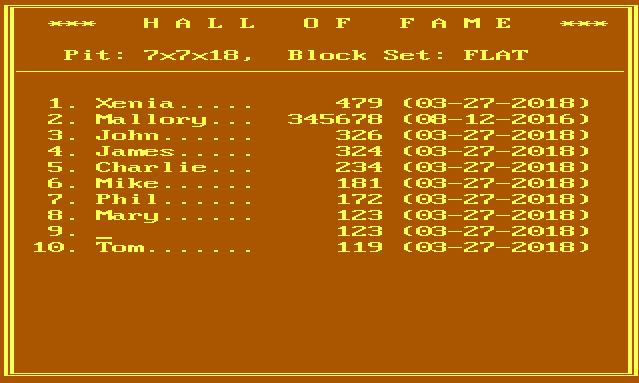
\includegraphics[width=0.7\textwidth]{advanced/550_more_structs/blockout/hs345678.png}
\caption{Table des meilleurs scores}
\end{figure}

Les deux premiers chiffres (1 et 2) ne sont pas affichés. Peut-être est-ce un problème
de formatage... mais le nombre est presque correct.
Maintenant, je le change en 999999 et relance le jeu:

\begin{figure}[H]
\centering
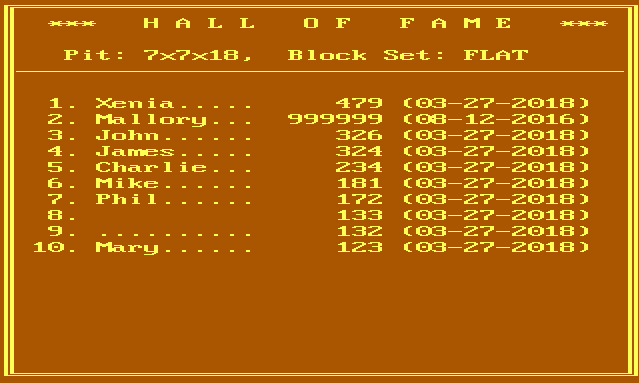
\includegraphics[width=0.7\textwidth]{advanced/550_more_structs/blockout/hs999999.png}
\caption{Table des meilleurs scores}
\end{figure}

Maintenant, c'est correct. Oui, la valeur du score est un entier 32-bit.

\subsubsection{Est-ce de la sérialisation?}

\dots presque.
Ce genre de sérialisation est très populaire dans les logiciels scientifiques et
d'ingénierie, où l'efficacité et la rapidité sont bien plus importantes que de convertir
de et vers \ac{XML} ou \ac{JSON}.

Une chose importante est que vous ne pouvez évidemment pas sérialiser des pointeurs,
car à chaque fois que vous chargez le programme en mémoire, toutes les structures
peuvent être allouées à des endroits différents.

Mais, si vous travaillez sur des sortes de \ac{MCU} à bas coût avec un simple \ac{OS}
dessus et que vous avez vos structures toujours allouées à la même place en mémoire,
peut-être pouvez-vous sauver et restaurer de la sorte.

\subsubsection{Bruit aléatoire}

Lorsque je préparais cet exemple, j'ai dû lancer \q{Block out} de nombreuses fois
et jouer un peu avec pour remplir la table des meilleurs scores avec des noms au
hasard.

Et lorsqu'il y avait seulement 3 entrées dans le fichier, j'ai vu ceci:

\begin{lstlisting}
00000000: 03 00 54 6f 6d 61 73 2e 2e 2e 2e 2e 00 da 2a 00  ..Tomas.......*.
00000010: 00 30 38 2d 31 32 2d 32 30 31 36 00 43 68 61 72  .08-12-2016.Char
00000020: 6c 69 65 2e 2e 2e 00 8b 1e 00 00 30 38 2d 31 32  lie........08-12
00000030: 2d 32 30 31 36 00 4a 6f 68 6e 2e 2e 2e 2e 2e 2e  -2016.John......
00000040: 00 80 00 00 00 30 38 2d 31 32 2d 32 30 31 36 00  .....08-12-2016.
00000050: 00 00 57 c8 a2 01 06 01 ba f9 47 c7 05 00 f8 4f  ..W.......G....O
00000060: 06 01 06 01 a6 32 00 00 00 00 00 00 00 00 00 00  .....2..........
00000070: 00 00 00 00 00 00 00 00 00 00 00 00 00 00 00 00  ................
00000080: 00 00 00 00 00 00 00 00 00 00 00 00 00 00 00 00  ................
00000090: 00 00 00 00 00 00 00 00 00 00 00 00 00 00 00 00  ................
000000a0: 00 00 00 00 00 00 00 00 00 00 93 c6 a2 01 46 72  ..............Fr
000000b0: 8c f9 f6 c5 05 00 f8 4f 00 02 06 01 a6 32 06 01  .......O.....2..
000000c0: 00 00 98 f9 f2 c0 05 00 f8 4f 00 02 a6 32 a2 f9  .........O...2..
000000d0: 80 c1 a6 32 a6 32 f4 4f aa f9 39 c1 a6 32 06 01  ...2.2.O..9..2..
000000e0: b4 f9 2b c5 a6 32 e1 4f c7 c8 a2 01 82 72 c6 f9  ..+..2.O.....r..
000000f0: 30 c0 05 00 00 00 00 00 00 00 a6 32 d4 f9 76 2d  0..........2..v-
00000100: a6 32 00 00 00 00                                .2....
\end{lstlisting}

Le premier octet a la valeur 3, signifiant qu'il y a 3 entrées.
Et ces 3 entrées sont présentes.
Mais nous avons des valeurs aléatoires dans la seconde moitié du fichier.

Le bruit provient probablement de données non initialisées.
Peut-être que \q{Block out} alloue de la mémoire pour 10 entrées quelque part dans
le \glslink{heap}{tas}, où, manifestement, des valeurs pseudo-aléatoires (laissées
par quelque chose d'autre) sont présentes.
Ensuite il a rempli les premier/second octet, 3 entrées, et puis n'a jamais touché
aux 7 autres entrées, donc elles ont été écrites dans le fichier telles quelles.

Lorsque \q{Block out} charge le fichier des meilleurs scores la fois suivante, il
lit le nombre d'entrée dans les 2 premiers octets (3) et puis ignore ce qui vient
après elles.

Ceci est un problème courant.
Pas un problème au sens strict: ce n'est pas un bogue, mais de l'information peut
fuiter à l'extérieur.

\myindex{Microsoft Word}
Les versions de Microsoft Word des années 1990 laissaient souvent des morceaux de
texte précédemment édité dans les fichiers *.doc*.
C'était alors une sorte de distraction d'obtenir un fichier \IT{.doc} de quelqu'un
d'autre, de l'ouvrir dans un éditeur hexadécimal et de lire d'autres choses, qui
avaient été éditées avant sur cet ordinateur.

\myindex{Heartbleed}
\myindex{OpenSSL}
Le problème peut être beaucoup plus sérieux: le bogue Heartbleed\footnote{\url{https://en.wikipedia.org/wiki/Heartbleed}}
dans OpenSSL.

\subsubsection{Devoir}

\q{Block out} a plusieurs types de pièces (plat/basique/étendu), la taille peut être configurée, etc.
Et il semble que pour chaque configuration, \q{Block out} a son propre tableau des
meilleurs scores.
J'ai remarqué que de l'information est probablement stockée dans le fichier \IT{BLSCORE.IDX}.
Ceci peut être un travail pour les fans de \q{Block out}---de comprendre aussi sa
structure.
Les fichiers de \q{Block out} sont ici: \url{http://beginners.re/examples/blockout.zip}
(incluant le fichier binaire des meilleurs scores que j'ai utilisé dans cet exemple).
Vous pouvez utiliser DosBox pour le lancer.

